The ModuTex system employs a multi-layered architecture designed for modularity, extensibility, and ease of use. This section details the implementation methodology and key design decisions.

\subsection{System Architecture}

The system consists of four primary components:

\begin{enumerate}
    \item \textbf{Environment Setup Scripts}: Automated installation and configuration tools for LaTeX distributions and language-specific packages.
    \item \textbf{Compilation Engine}: Streamlined build process using latexmk with XeLaTeX backend for Unicode and font support.
    \item \textbf{AI Integration Layer}: Python-based CLI tool for content generation and citation management.
    \item \textbf{Template System}: Modular template collection for different publication venues.
\end{enumerate}

\subsection{Implementation Details}

\subsubsection{Automated Environment Setup}

The environment setup process uses shell scripting with OS detection to ensure compatibility across Linux, macOS, and Windows Subsystem for Linux (WSL). The scripts implement robust error handling and provide colored output for enhanced user experience.

\subsubsection{AI-Powered Content Generation}

The texchat.py tool integrates with OpenAI's GPT-4 API to provide intelligent content generation capabilities. The system uses carefully crafted prompts to ensure LaTeX-compatible output with proper citation formatting.

\subsubsection{Citation Management}

Automatic citation fetching leverages the CrossRef API to retrieve BibTeX entries from DOI references. This eliminates manual citation formatting and ensures accuracy in bibliographic data.

\subsection{Language Support}

The system provides comprehensive support for both English and Persian languages, with automatic font configuration and proper bidirectional text handling. Figure \ref{fig:sample2} illustrates the language selection workflow, ensuring proper rendering regardless of the chosen language.

\begin{figure}[htbp]
    \centering
    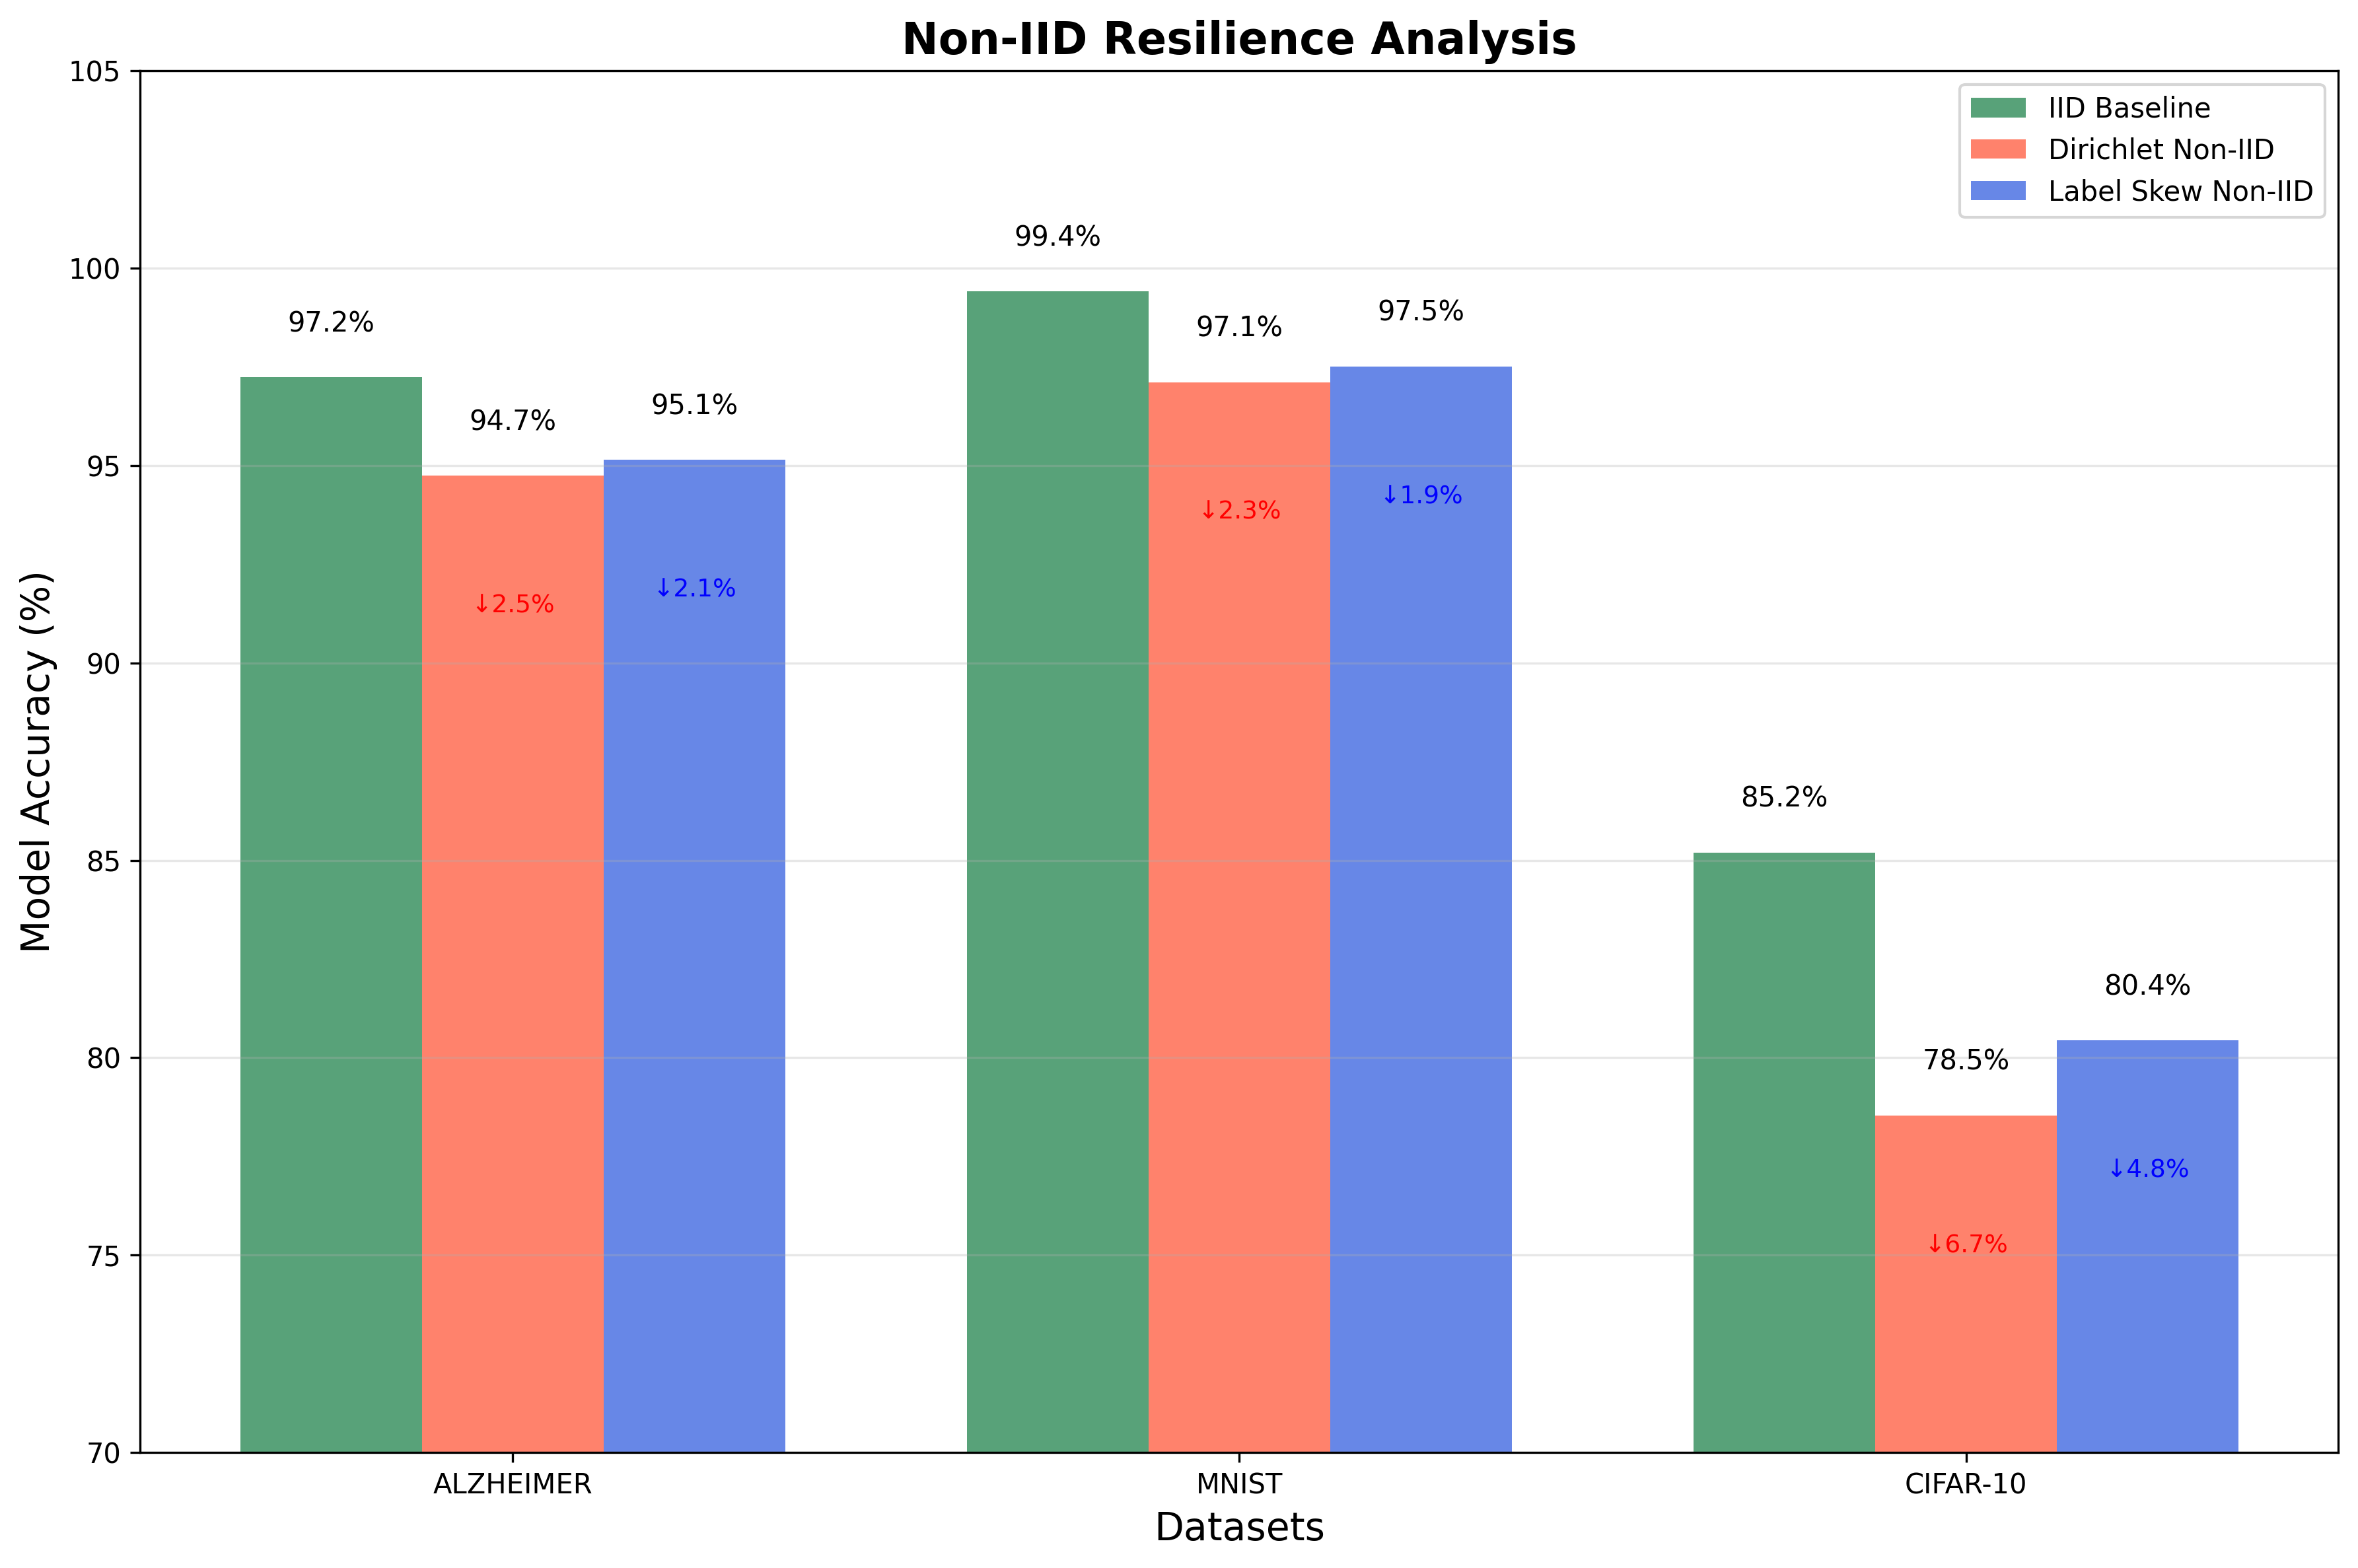
\includegraphics[width=0.6\textwidth]{figures/fig2.png}
    \caption{Language configuration and font selection process}
    \label{fig:sample2}
\end{figure} 